\section{Enumerating the Interpolants in $\F_2[A,B,C]$}
\label{sec:alg}
Lemma~\ref{noofinter} gives us the number of interpolants that exist for the given pair 
$(J_A,J_B)$. This section presents procedures for
enumerating these interpolants using $SM(J_D)$. 
Note that these procedures can only be applied while operating over 
the field $\F_2$. First we describe a procedure for enumerating all the interpolants.
This is made possible by exploiting the relationship between 
the interpolants and $SM(J_D)$.
\begin{Theorem}
\label{thm:enum_all}
Given the interpolant setup over $\F_2[A,B,C]$, let $SM(J_D) =\{m_1,\dots,m_l\}$. 
Construct a polynomial $f_i$ 
using any linear combination of $\{m_1,\dots,m_l\}$ as, 
\begin{equation}
\label{eqn:fi}
f_i = \lambda_1\cdot m_1 + \lambda_2\cdot m_2 +\cdots+ \lambda_l\cdot m_l
\end{equation} 
where each $\lambda_j \in \mathbb{F}_2 =  \{0,1\}$.
Then all the ideal-interpolants $J_I$ can be obtained as,
\begin{equation}
\label{eqn:ji}
J_I = J_S\cdot(J_D + \langle f_i \rangle).
\end{equation}
% where $\langle f_i \rangle$ is the ideal generated by the polynomial $f_i$.
\end{Theorem}
There can be $2^l$ such $f_i$, and as $|SM(J_D)| = l$, the number of interpolants
is also $2^l$. Therefore, each $f_i$ in Eqn.~(\ref{eqn:ji}) will result in a distinct interpolant.

\begin{proof}

We want to prove that each $f_i$ will result in a 
distinct interpolant when used in Eqn.~(\ref{eqn:ji}). Consider the variety $\Vc(J_D)$
and its cardinality $|\Vc(J_D)| = l$. From the proof of Lemma~\ref{noofinter}, we know that
the union of the variety $\Vc(J_S)$ and each subset of  $\Vc(J_D)$ produces a new 
interpolant. Therefore
\begin{equation}
\label{eqn:jsuwi}
\Vc(J_I) = \Vc(J_S) \cup W_i 
\end{equation}
where $W_i \in PowerSet(\Vc(J_D))$.
\begin{figure}[hbt]
\centering
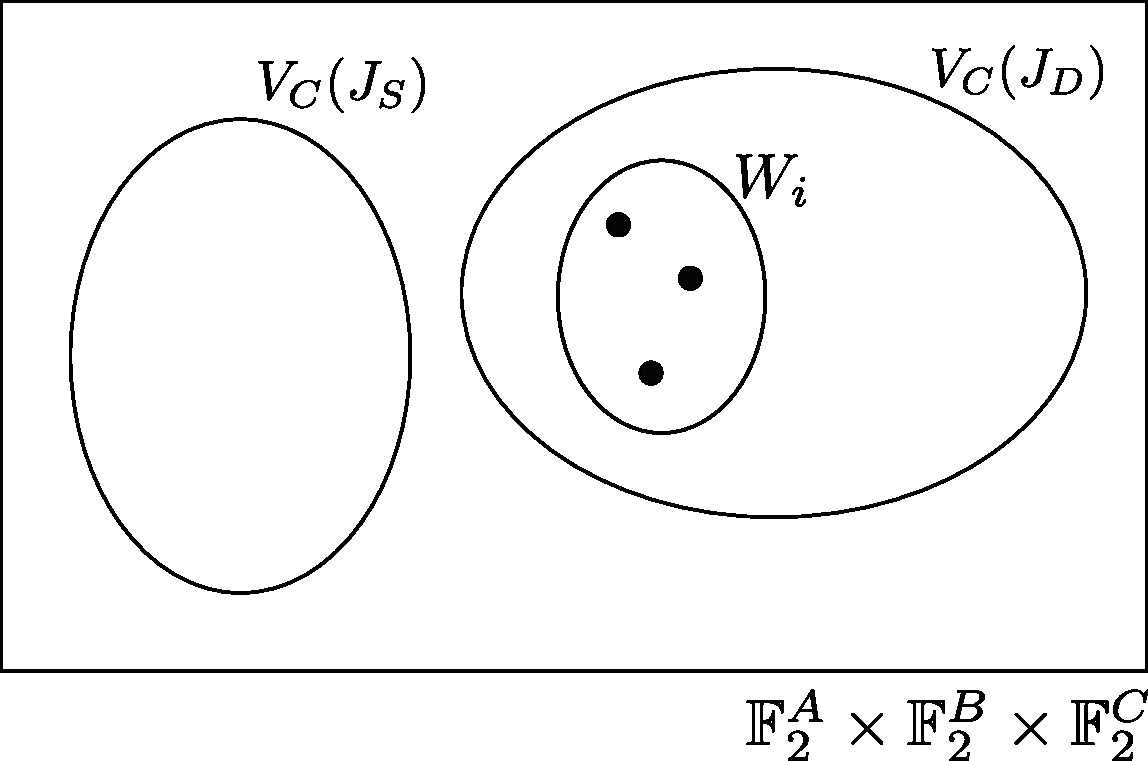
\includegraphics[scale=0.30]{vjd.pdf}
\caption{The variety $\Vc(J_D)$ and an element $W_i$ in its power set.}
\label{Fig:vjd}
\end{figure}  
\par Every $W_i$ is a set of finite number of points as shown in Fig.~\ref{Fig:vjd}, and 
therefore it forms a variety. As we are working over finite fields, the ideal of this variety 
can be constructed using only one polynomial $f'_i$. For example, $f'_i$ could be constructed by
means of Lagrange's interpolation formula over $W_i$. Therefore,
$\Vc(\langle f'_i \rangle) = W_i$. Note that there can be multiple polynomials
$f'_i$ with variety $W_i$ and they belong to the same equivalence class of polynomials
$\pmod{J_D}$. Consider the reduction $f'_i \xrightarrow{GB(J_D)} f_i$. Then
$\Vc(J_D+\langle f'_i \rangle) = \Vc(J_D + \langle f_i \rangle)$.
As $\Vc(\langle f'_i \rangle) = \Vc(J_D + \langle f'_i \rangle)$ because $\Vc
(\langle f'_i \rangle) \subseteq \Vc(J_D)$, we have $\Vc(\langle f'_i \rangle) =
\Vc(J_D + \langle f_i \rangle) = W_i$.

As $f'_i$ is reduced by 
$GB(J_D)$, the remainder $f_i \in \Fq[C]/J_D$ is a canonical representative 
for the equivalence class containing
$f'_i$ and is composed of only $SM(J_D)$. 

\par There are $2^l$ such equivalence classes of polynomials $\pmod{J_D}$ and each one of 
them can be reduced to a unique $f_i$. As there are $l$ standard monomials
$\{m_1,\dots,m_l\}$, they can be combined linearly to form $2^l$ unique polynomials $f_i$. 
Each equivalence class corresponds to a distinct interpolant (Eqn.~(\ref{eqn:jsuwi})). 
Consequently each $f_i$ will also correspond to a distinct interpolant,

\begin{align*}
\Vc(J_I) &= \Vc(J_S) \cup W_i ~~~(\text{from Eqn.~(\ref{eqn:jsuwi})}) \\
\Vc(J_I) &= \Vc(J_S) \cup (\Vc(J_d+\langle f_i \rangle)) \\
\Vc(J_I) &= \Vc(J_S) \cup (\Vc(J_d)\cap \Vc(\langle f_i \rangle)) \\
J_I &= J_S \cdot (J_D + \langle f_i \rangle) ~~~ (\text{using ideal-variety duality})
\end{align*} 

\end{proof}

\begin{Example}
\label{ex:enuall}
{\it
From Example~\ref{ex:main} and \ref{ex:jd} that are setup over $\F_2[A,B,C]$, 
we have $J_S = \langle cd, b + d+ 1 \rangle$ 
and $J_D = \langle d+1,bc+b+c+1 \rangle$ with
$SM(J_D) = \{1,b,c\}$. We can enumerate all the interpolants for the pair $(J_A,J_B)$ using
$f_i = \lambda_1\cdot 1 + \lambda_2\cdot b + \lambda_3\cdot c$ 
where $\{\lambda_1,\lambda_2,\lambda_3\} \in \{0,1\}$. 
\begin{itemize}
	\item Let $f_1 = c$ with $(\lambda_1,\lambda_2,\lambda_3)=(0,0,1)$.\\
	The GB computation 
	of the ideal $J_S\cdot (J_D + \langle f_1 \rangle)$ results in 
	$\langle cd,bd+b+d+1,bc+cd+c \rangle$ ~~ (= $J_1$ from Example~\ref{ex:main}) 
	\item Let $f_5 = b+1$ with $(\lambda_1,\lambda_2,\lambda_3)=(1,1,0)$. \\
	The GB computation 
	of the ideal $J_S\cdot (J_D + \langle f_5 \rangle)$ results in 
	$\langle bc+c,bd+b+d+1 \rangle$ ~~ (= $J_5$ from Example~\ref{ex:main})
	\item Let $f_6 = b+c+1$ with $(\lambda_1,\lambda_2,\lambda_3)=(1,1,1)$. \\
	The GB computation 
	of the ideal $J_S\cdot (J_D + \langle f_6 \rangle)$ results in 
	$\langle bd+b+d+1,bc+cd+c \rangle$ ~~ (= $J_6$ from Example~\ref{ex:main})
	\item Similarly, all the 8 interpolants can be obtained from the
	8 possible $f_i$.
\end{itemize}
}
\end{Example}

The reason why Theorem~\ref{thm:enum_all} requires the interpolant setup over $\F_2[A,B,C]$ is as follows.
If we assume that the setup was over some other finite field $\Fq$, then Eqn.~(\ref{eqn:fi}) will 
produce $q^l$ $(l=|SM(J_D|)$ polynomials $f_i$. However, the number of interpolants is exactly equal 
to $2^l$ irrespective of the field we are working on (Lemma~\ref{noofinter}). As a result, multiple 
$f_i$ can produce same interpolant unlike the case when $q=2$ (each $f_i$ produces a distinct interpolant).
The study to enumerate all the interpolants for any finite field using the $SM(J_D)$ 
is a part of our future work.


\par In practice, we don't need to compute all interpolants. However, given an interpolant it may
be desirable to obtain a larger interpolant that provides a better abstraction.
Given an ideal-interpolant $J_I$ we discuss how a larger 
ideal-interpolant $J_K$ can be obtained so that $\Vc(J_I) \subset \Vc(J_K)$.

\par Let $J_I$ and $J_K$ be two ideal-interpolants obtained using polynomials
$f_i$ and $f_k$ respectively (using Eqn. (\ref{eqn:ji})). Assuming that 
$\Vc(J_I) \subset \Vc(J_K)$ consider,
\begin{align*}
\Vc(J_I) &\subset \Vc(J_K) \\
\Vc(J_S\cdot(J_D + \langle f_i \rangle)) &\subset \Vc(J_S\cdot(J_D + \langle f_k \rangle)) \\ 
\Vc(J_S) \cup \Vc(J_D + \langle f_i \rangle) &\subset \Vc(J_S) \cup \Vc(J_D + \langle f_k \rangle)
\end{align*}
\par \noindent as the sets $\Vc(J_S)$ and $\Vc(J_D)$ are disjoint (Fig.~\ref{Fig:vjd}) we can
write
\begin{align*}
\label{eqn:chainofinter}
\Vc(J_D + \langle f_i \rangle) &\subset \Vc(J_D + \langle f_k \rangle) \\
I(\Vc(J_D + \langle f_i \rangle)) &\supset I(\Vc(J_D + \langle f_k \rangle)) 
\end{align*}
using Lemma~\ref{lemma:radical-ff} and Theorem~\ref{thm:strong-ns} we have
\begin{align}
\begin{split}
J_D + \langle f_i \rangle &\supset J_D + \langle f_k \rangle \\
J_D + \langle f_i \rangle &\supset f_k
\end{split}
\end{align}  
% If the interpolant $\Vc(J_i)$ is contained in some other interpolant 
% computed using  $f_j$, then the relation in Eqn.~\ref{eqn:chainofinter} 
% is also true for that $f_j$. 
\par Now that we know that $f_k$ is contained in $J_D + \langle f_i \rangle$,
we will show how $f_k$ can be obtained from the GB of $J_D + \langle f_i \rangle$.

\begin{Theorem}
\label{thm:chainofinter}
Given an ideal-interpolant $J_I$ computed as $J_I = J_S\cdot(J_D + \langle f_i \rangle)$. Obtain the
reduced $GB$ $G_{Di}=GB(J_D + \langle f_i \rangle)$. Then there must exist 
at least one $g_j \in
G_{Di}$ which is a linear combination of $SM(J_D)$. 
Each $g_j \neq f_i$ can be used to 
obtain a new interpolant $J_K$ such that
$\Vc(J_I) \subset \Vc(J_K)$.  
\end{Theorem}

\begin{proof} 
We need to show that $G_{Di}$ will contain 
at least one polynomial that is a  linear combination of $SM(J_D)$.
As a reduced $GB$ is a canonical representation, $G_{Di}$ 
can also be computed as $GB(GB(J_D) + \langle f_i \rangle)$. 
Consider the set $GB(J_D)$
where each polynomial $p_r$ can be written as $lt(p_r) + (p_r - lt(p_r))$. 
The monomials in $p_r-lt(p_r)$ can only contain the elements of $SM(J_D)$ 
(otherwise they can be divided by the leading terms of polynomials in $J_D$).

\par Construct $GB(J_D) + \langle f_i \rangle$ and compute the 
reduced $GB$ of this ideal. As the set of polynomials $GB(J_D)$ is already a 
$GB$, Buchberger's algorithm will pair $f_i$ and each polynomial from the set
$GB(J_D)$ for the $S$-$poly$ computation $S$-$poly(p_r,f_i) \xrightarrow{GB(J_D),f_i}_+ h_r$. 
The $S$-$poly$ is reduced modulo $\{GB(J_D), f_i\}$ 
and as a result $h_r$ will only be composed of $SM(J_D)$. 
% If the reduced S-poly 
% contains some monomials $\not \in SM(J_D)$, then they will be reduced by some 
% polynomial in $GB(J_D)$. 
This implies that there will be at least one polynomial
in the $GB(J_D + \langle f_i \rangle))$ containing monomials only from the set $SM(J_D)$. 
This polynomial can then be used to compute an ideal-interpolant $J_K$ such that 
$\Vc(J_I) \subset \Vc(J_K)$.

% Let's say we perform the S-poly computation for some $p_r$ and $f_i$. This will result
% in an expression like $\beta \cdot tail(p_r) + \alpha \cdot tail(f_i)$ where 
% $\alpha = LCM(lt(f_i),lt(p_r))/lt(f_i)$ and $\beta  = LCM(lt(f_i),lt(p_r))/lt(p_r)$. This S-poly 
% is then reduced modulo each polynomial $p_r$ and $f_i$. The monomials of this remainder can
% only be elements from $SM(J_D)$ and can be used to obtain a larger interpolant (Eqn.~\ref{eqn:ji}).  
% Also there always be at least one such polynomial otherwise it would imply $f_i \in J_D$ ($i.e.$ all the S-poly are zero).
% This is not possible as $f_i$ is constructed using the $SM(J_D)$. If there is only one polynomial
% in $G_{Di}$ which is a linear combination of $SM(J_D)$ and is $f_i$ itself, then using 
% this polynomial in Eqn.~\ref{eqn:ji} will result in $f_i$ itself. In that case, the only larger interpolant
% is $J_L$ itself.   
% \end{proof}

\end{proof}

If there is only one polynomial
in $G_{Di}$ which is a linear combination of $SM(J_D)$ and is $f_i$ itself, then using 
this polynomial in Eqn.~(\ref{eqn:ji}) will result in $J_I$ itself. In that case, 
the only larger interpolant is $J_L$.

\par Theorem \ref{thm:chainofinter} gives an approach to devise an algorithm that computes a chain of progressively larger interpolants starting from $J_S$. The following steps explain the algorithm.
\begin{enumerate}
	\item Given the pair $(J_A,J_B)$ in $\F_2[A,B,C]$, compute $J_S$, $J_D$, 
	and $SM(J_D)$. Store $J_S$ in some list $L$.
	\item Pick a polynomial $f_i = \sum_{i=1}^{i=l} \lambda_i \cdot m_i$, 
	where $\{m_1, \dots,m_l\} = SM(J_D)$ and $\lambda_i \in \{0,1\}$. ($f_i \neq 1$ otherwise,
	$GB(J_D + \langle 1 \rangle) =1$, so $J_I = J_S$).
	\item Compute $G_{Di} = GB(J_D + \langle f_i \rangle)$. Append $J_I = J_S\cdot G_{Di}$
	to $L$.
	\item In $G_{Di}$ find polynomials $g_j$ which are of the 
	form $\sum_{i=1}^{i=l} \lambda_i \cdot m_i$.
	\item Pick a $g_j \neq f_i$ and goto step 3 where $g_j$ replaces $f_i$
	in the computation of $G_{Di}$.
	\item If in step 4, there is only one $g_j$ and $g_j = f_i$,
	terminate the algorithm after appending $J_L = J_S \cdot J_D$ to $L$.
\end{enumerate} 
The algorithm returns the list $L$ whose first element is $J_S$ and last element is
$J_L$ with a chain of progressively larger interpolants in between.
The pseudo-code for this algorithm is presented in Algorithm~\ref{algo:chainofinter}. 


% The inputs are the ideals $J_S$, $J_D$, and the polynomial $f_i$. 
% The algorithm initializes a list $L$ that will store the interpolants computed by the algorithm. The infinite while 
% loop terminates when there is only one $g_j$ in $G_{Di}$ and $g_j = f_i$. In that case, the algorithm appends
% $J_L = J_S\cdot J_D$ to $L$ and returns $L$. Otherwise, it picks one $g_j$, appends the corresponding ideal-interpolant 
% to $L$ and re-iterates with $G_{Di} = GB((J_D + \langle g_j \rangle))$.

\begin{algorithm}
\caption{Compute larger ideal-interpolants given $J_I \neq J_S$}
\label{algo:chainofinter}
\begin{algorithmic}[1]

\Procedure{$get\_larger\_interpolant$}{$J_S,J_D,SM(J_D)$}
\State {\it Initialize list $L$ for storing interpolants}
\State {\it Append $J_S$ to $L$}
\State {\it Pick $f_i = \sum_{i=1}^{i=l} \lambda_i \cdot m_i ~~~ (f_i\neq 1)$}
\While{(1)}
\State Compute $G_{Di} = GB(J_D + \langle f_i \rangle)$ 
\State {\it Append $J_S\cdot G_{Di}$ to $L$}
\State {\it Find $g_j \in G_{Di}$ $s.t.$ $g_j = \sum_{i=1}^{i=l} \lambda_i \cdot m_i$}
\If{\it $|\{g_j\}| = 1$ and $g_j = f_i$}
\State {\it Append $J_S\cdot J_D$ to $L$}
\State \Return $L~~$ {\it //Reached largest interpolant}
\Else
\State {\it Choose a $g_j \neq f_i$}
\State {\it $f_i = g_j$}
% \State $G_{Di} = GB(J_D + \langle g_j \rangle)$
\EndIf

\EndWhile
% \State \Return $L$
\EndProcedure

\end{algorithmic}
\end{algorithm}

\begin{Example}
\label{ex:chainofinter}
{\it
The algorithm can be understood with this example. Consider the following steps.
\begin{itemize}
	\item From Example \ref{ex:jd}, $J_S = \langle cd, b + d+ 1 \rangle$,
	$J_D = \langle d+1,bc+b+c+1 \rangle$ with $SM(J_D) = \{1,b,c\}$. The ideal-interpolant $J_S$
	is appended to $L$ so that $L = [J_S]$.
	
	\item We need to pick a $f_i = \lambda_1\cdot 1 + \lambda_2\cdot b + \lambda_3\cdot c$ and
	$f_i \neq 1$. Let $f_1 = c$ with $(\lambda_1,\lambda_2,\lambda_3) = (0,0,1)$.
	
	\item The computation $G_{Di} = GB(J_D + \langle f_1 \rangle)$ results in the ideal
	$G_{Di} = \langle d+1,b+1,c \rangle$. The ideal-interpolant $J_1 = J_S \cdot G_{Di}$ 
	(same as the $J_1$ in Example~\ref{ex:enuall}) is appended to 
	$L$ so that $L = [J_S,J_1]$.
	
	\item In $G_{Di}$, the only $g_j$ of the form $\sum_{i=1}^{i=l} \lambda_i \cdot m_i$ are
	$g_1 = b+1$ and $g_2 = c$. 

	\item We select $g_1$ for the computation of larger interpolant as $g_2 = f_1$. Notice that $g_1$ is equal to $f_5$ from Example ~\ref{ex:enuall}.
	
	\item Using $g_1$ in the computation $GB(J_D + \langle g_1 \rangle)$ results in the
	ideal $\langle d+1, b+1\rangle$. Also the ideal-interpolant $J_5 = J_S\cdot (J_D + \langle g_1 
	\rangle) = J_S\cdot (J_D + \langle f_5) \rangle$ is appended to $L$ so that $L = [J_S,J_1,J_5]$.
	
	\item The only $g_i$ in $GB(J_D + \langle g_1 \rangle) = \langle d+1, b+1\rangle$ of the 
	form $\sum_{i=1}^{i=l} \lambda_i \cdot m_i$ is $b+1$. As $b+1 = f_5$, the only larger
	interpolant for $J_5$ is $J_L$. Therefore, the algorithm returns the $L = [J_S,J_1,J_5,J_L]$.

\end{itemize}
% From Example~\ref{ex:main}, we have $\Vc(J_1) \subset \Vc(J_5)$ and $\Vc(J_1) \subset \Vc(J_6)$. From 
% Example~\ref{ex:enuall}, we also know that $f_1 = c,~f_5 = b+1,$ and $f_6 = b + c + 1$ and the ideal $J_D$. 
% The computation $GB(J_D + \langle f_1 \rangle)$ results in the ideal $\langle d+1,b+1,c \rangle$. We have
% $g_1 = b+1$ and $g_2 = c$ as linear combinations of $SM(J_D)$. Notice that $g_1 = f_5$ and performing
% the computation $J_S\cdot(J_D + \langle g_1 \rangle)$ will result in $J_5$. Also $g_2 = f_1$, so we will
% not consider it in the computation of a larger interpolant. However, the linear combination $g_1 + g_2 = f_6$
% is also a suitable candidate for obtaining a larger interpolant and results in $J_6$.
% \par The computation $J_D + \langle f_5 \rangle$ results in $\langle d+1, b+1\rangle$. We only have one $g_1$
% as linear combinations of $SM(J_D)$ and $g_1 = f_5$. Therefore, the only larger interpolant for $\Vc(J_5)$ is
% $J_L$. Same is also true for $J_6$.

}

\vspace{0.1in}
\end{Example}

%% \par \noindent \underline{Discussions:} 
%% \begin{itemize}
%% \item The theorems and algorithm presented 
%% in the sections \ref{sec:theory} and \ref{sec:alg} make use of Gr\"obner basis concepts
%% and rely on GB computation. The computational complexity of
%% Buchberger's algorithm is exponential making these theorems practically infeasible. 
%% \par GB concepts are being extensively used in the verification of hardware circuits. 
%% When operating over Boolean circuits, \cite{pruss:tcad} and \cite{xiaojun:hldvt2016}
%% describe a topological monomial order that can be 
%% derived from the gates of the circuit. This order obviates the need to explicitly compute a 
%% Gr\"obner basis and the overall complexity is dictated by polynomial reductions. 
%% \par We are currently working on orderings and heuristics that can avoid GB computation complexity
%% when the Craig interpolants are used for circuit based applications like logic synthesis.
%% However, before these techniques can be applied to circuits, a theory of
%% Craig interpolants in finite fields needs to be set in place which 
%% is the primary purpose of this paper.

%% \item As an improvement to our approach, the step in line 13 of Algorithm~\ref{algo:chainofinter} can use improved heuristic 
%% when choosing a $g_j$. Instead of selecting just one $g_j$ of the form $\sum_{i=1}^{i=l} \lambda_i \cdot m_i$,
%% one can also select a linear combination of multiple $g_j$ as long as this combination does not
%% compute to $f_i$. This is because the combination of multiple $g_j$ is still of the
%% form $\sum_{i=1}^{i=l} \lambda_i \cdot m_i$. 
%% \par From Example \ref{ex:main} we know that $\Vc(J_1) \subset \Vc(J_5)$
%% and $\Vc(J_1) \subset \Vc(J_6)$. We also saw in the Example \ref{ex:chainofinter} that we can
%% obtain $J_5$ by selecting $g_1 = b+1$ from the set $GB(J_D + \langle f_1 \rangle)$. If we consider the linear 
%% combination $g_3$ of $g_1$ and $g_2$ obtained as $g_3 = g_1 + g_2 = b+c+1$, then from Example \ref{ex:enuall},
%% $g_3 = f_6$ and can be used to compute $J_6$. 

%% \end{itemize} 

% \begin{Theorem}
% Given an ideal-interpolant $I_j$ computed using the Theorem~\ref{enum_all} and the polynomial
% $f_j$ (linear combination of $SM(J_D)$,
% \begin{enumerate}
% 	\item Compute reduced $GB$ of $(J_D + \langle f_j \rangle)$
% 	\item The $GB(J_D + \langle f_j \rangle)$ will contain some 
% 	polynomials $h_1,\dots,h_r$ that are linear combinations of
% 	$SM(J_D)$. 
% 	\item Use Theorem~\ref{enum_all} and each of these $h_i$
% 	or their linear combinations to obtain interpolants that contain 
% 	$\Vc(I_j)$.
% \end{enumerate}
% \end{Theorem}
% After obtaining a larger ideal-interpolant $I_k$ we can using this
% theorem again to obtain an interpolant which is larger than $\Vc(I_k)$.
% We may encounter a $h_i$ exactly equal to $f_j$ (the polynomial 
% used for computing $I_j$). We will avoid using this $h_i$ as it will
% result in $I_j$ itself.  
